\documentclass[portrait]{article}
%\documentclass[landscape]{article}
\usepackage[utf8x]{inputenc}
\usepackage[T1]{fontenc}
\usepackage{amsmath}
\usepackage{graphicx}
\begin{document}

\input{title-tmp.tex} % should contain author, etc.

\maketitle

\begin{abstract}
Atliktas darbas pateiktas pav.~\ref{fig-report}.
\end{abstract}

% ---------------------------
\begin{figure}[b]
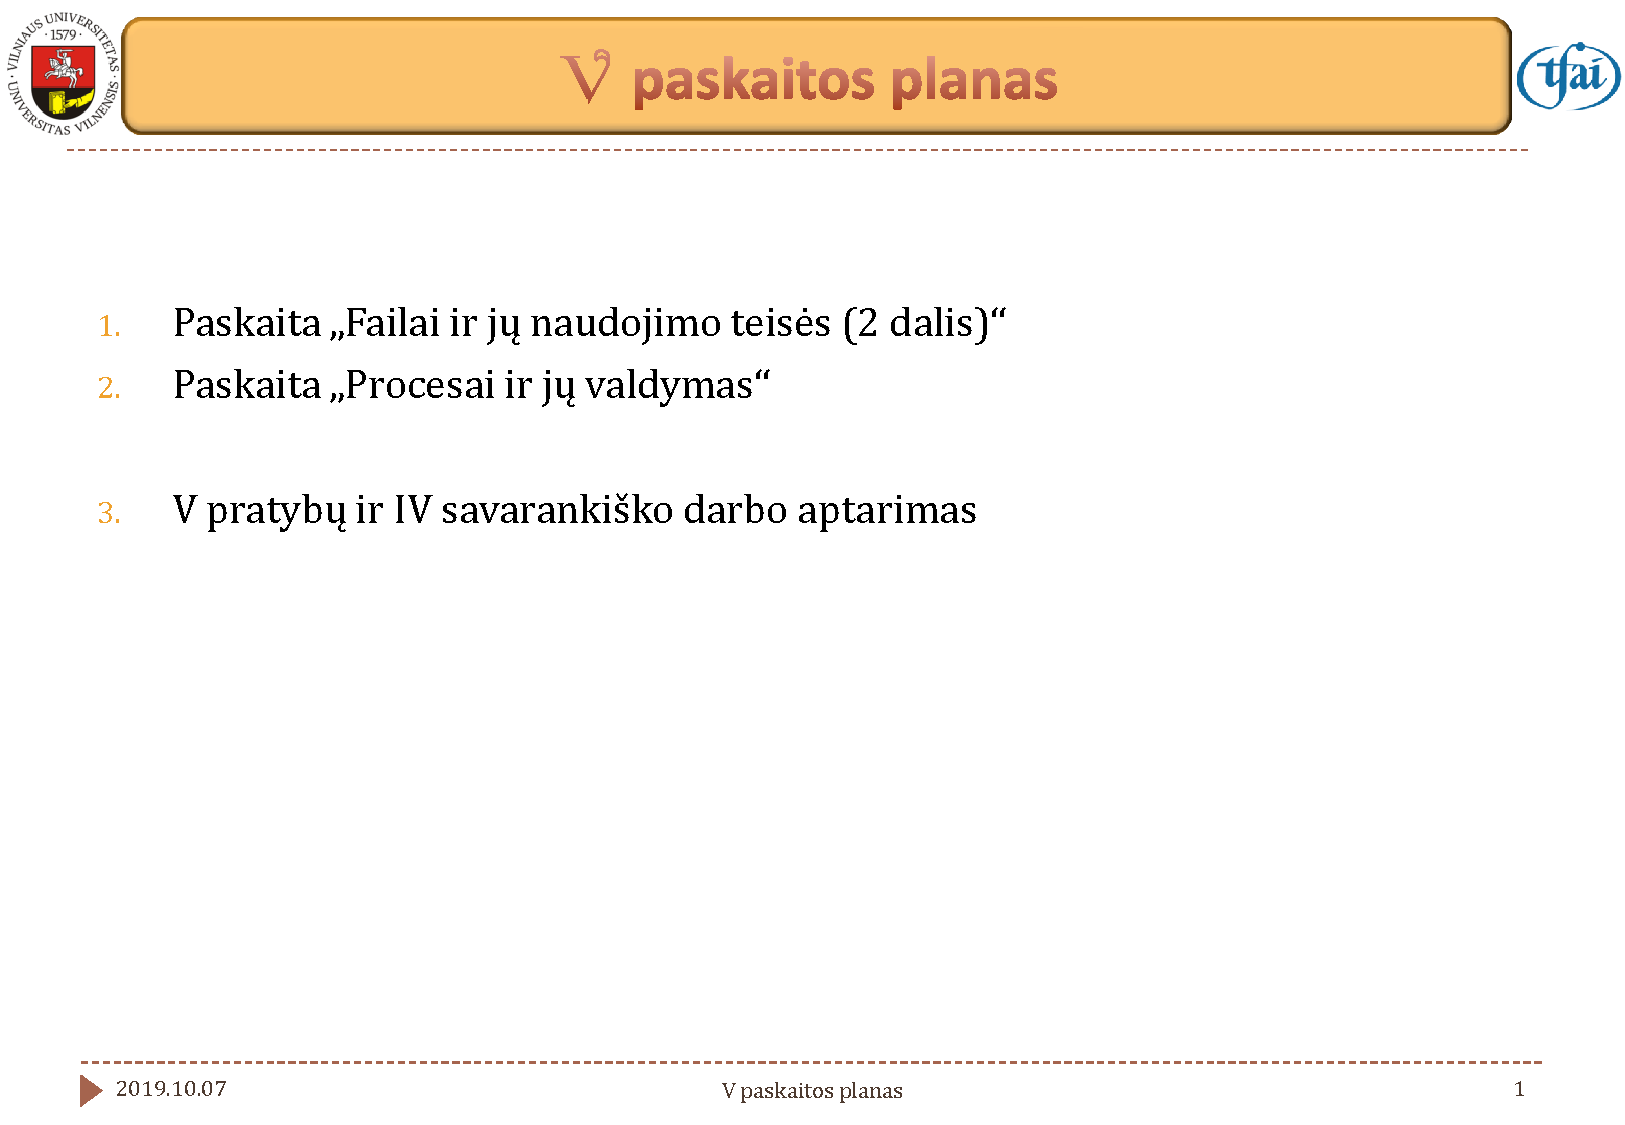
\includegraphics[height=0.8\textheight,width=0.9\textwidth]{pavyzdys.pdf}
\caption{Atlikto darbo pirmasis puslapis.}
\label{fig-report}
\end{figure}
% ---------------------------

\end{document}
